% !TEX root = tracking.tex
\section{10D Quadrotor RRT Example \label{sec:results}}
\textcolor{red}{explain 10D computation, RRT planning and conversion to dynamics, putting the two together, results}
\subsection{10D}
\textcolor{red}{use decomposition to run this in 10D. Follows 3D super-simple dynamics. Parameters, results}
\begin{figure*}
	\centering
	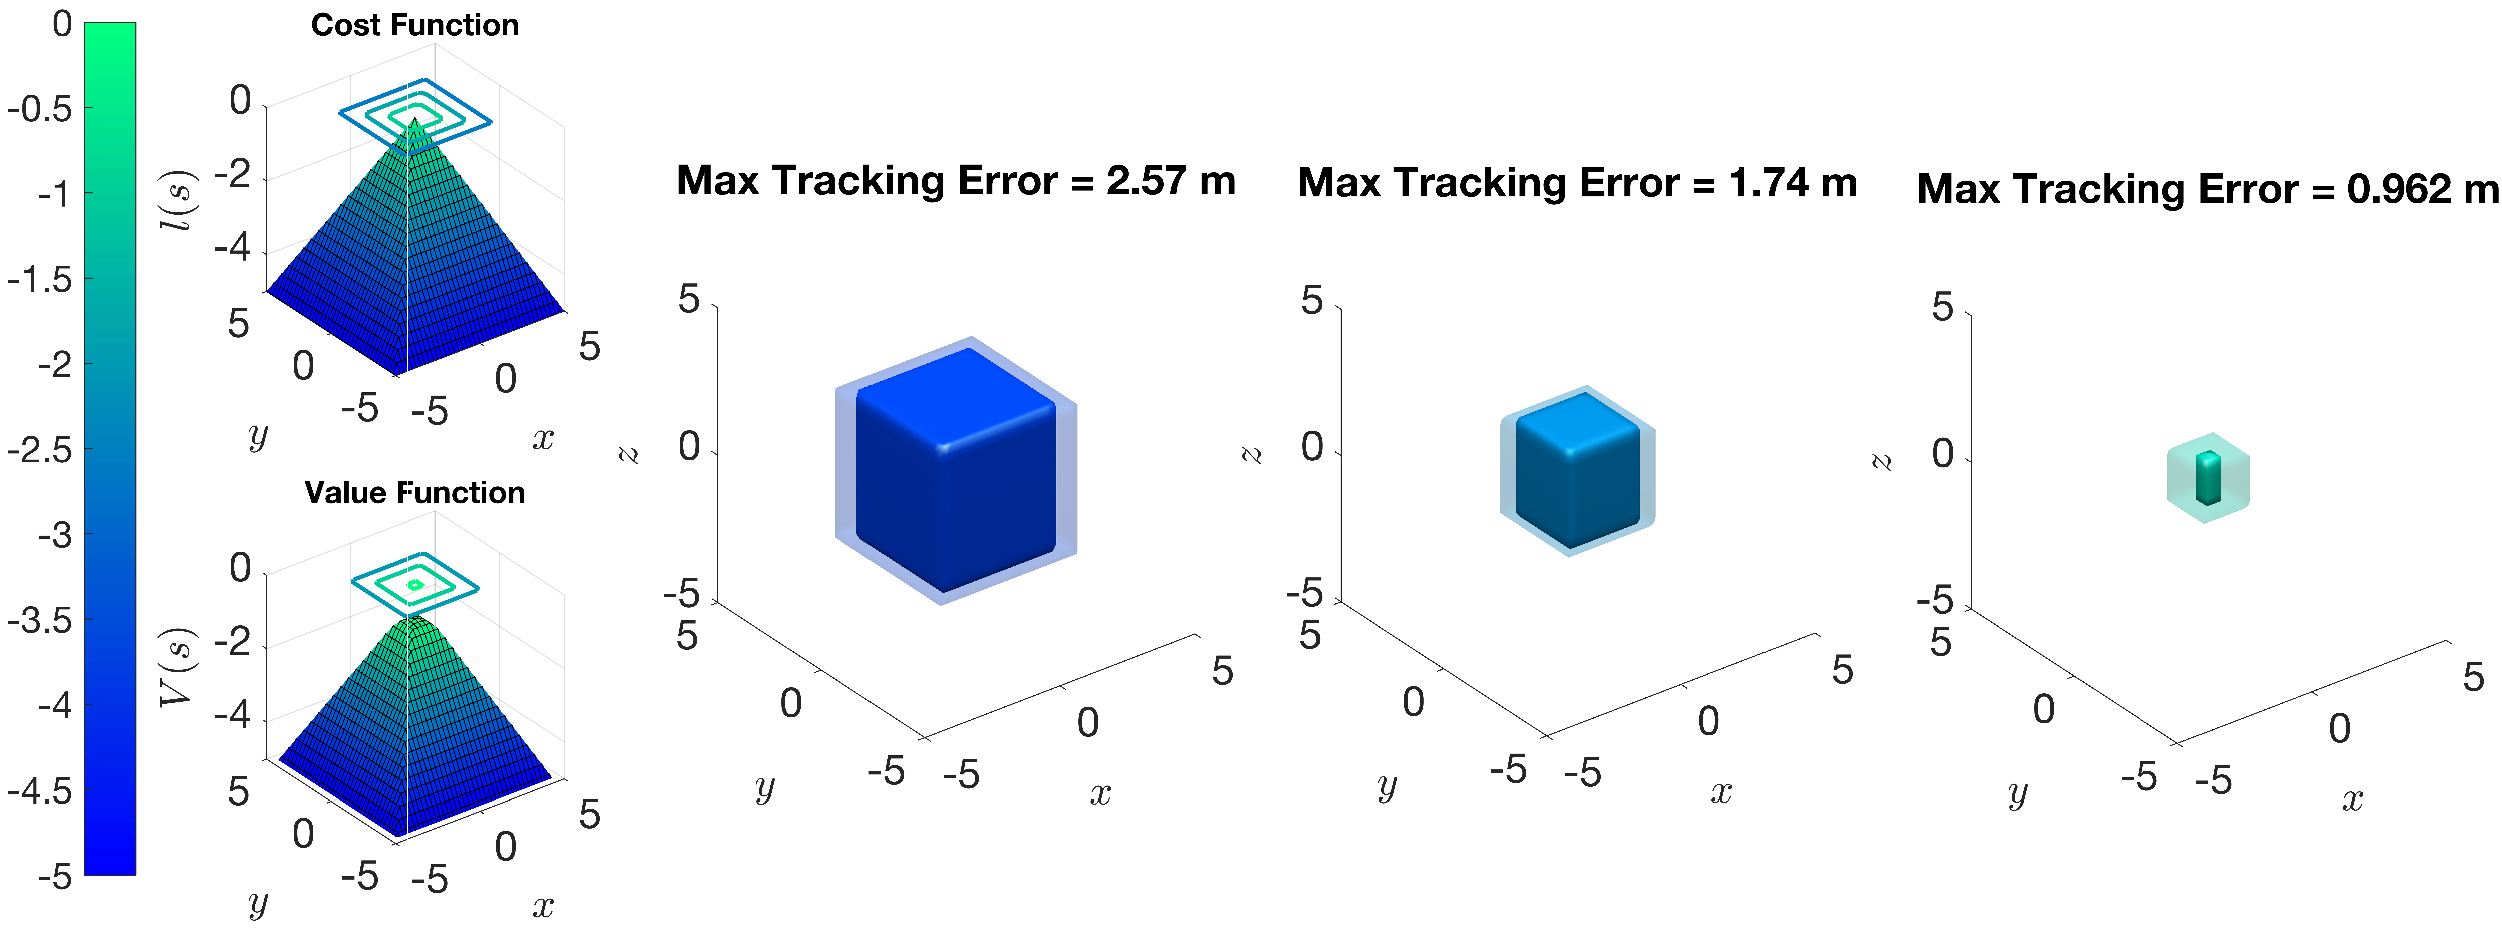
\includegraphics[width=0.8\textwidth]{fig/quad10D_example2}
	\caption{\textcolor{red}{2D projections of reward and value functions, along with corresponding 3D positional projections of initial state and tracking error bound}}
	\label{fig:quad10D_example}
\end{figure*} 
\subsection{RRT Online Planning}
\textcolor{red}{what RRT planner we're using, how we convert it to dynamics, setup of environment, results}